%%%%%%%%%%%%%%%%%%%%%%%%%%%%%%%%%%%%%%%%%
% Programming/Coding Assignment
% LaTeX Template
%
% This template has been downloaded from:
% http://www.latextemplates.com
%
% Original author:
% Ted Pavlic (http://www.tedpavlic.com)
%
% Note:
% The \lipsum[#] commands throughout this template generate dummy text
% to fill the template out. These commands should all be removed when 
% writing assignment content.
%
% This template uses a Perl script as an example snippet of code, most other
% languages are also usable. Configure them in the "CODE INCLUSION 
% CONFIGURATION" section.
%
%%%%%%%%%%%%%%%%%%%%%%%%%%%%%%%%%%%%%%%%%

%----------------------------------------------------------------------------------------
%	PACKAGES AND OTHER DOCUMENT CONFIGURATIONS
%----------------------------------------------------------------------------------------

\documentclass{article}

\usepackage{fancyhdr} % Required for custom headers
\usepackage{lastpage} % Required to determine the last page for the footer
\usepackage{extramarks} % Required for headers and footers
\usepackage[usenames,dvipsnames]{color} % Required for custom colors
\usepackage{graphicx} % Required to insert images
\usepackage{listings} % Required for insertion of code
\usepackage{courier} % Required for the courier font
\usepackage{lipsum} % Used for inserting dummy 'Lorem ipsum' text into the template
\usepackage[utf8]{inputenc} % Required for inputting international characters
\usepackage[T1]{fontenc} % Output font encoding for international characters
\usepackage{pdfpages}

% Margins
\topmargin=-0.45in
\evensidemargin=0in
\oddsidemargin=0in
\textwidth=6.5in
\textheight=9.0in
\headsep=0.25in

\linespread{1.1} % Line spacing

% Set up the header and footer
\pagestyle{fancy}
\lhead{\hmwkTitle} % Top left header
\rhead{\hmwkAuthorName} % Top right header
%\chead{\hmwkClass\ (\hmwkClassInstructor\ \hmwkClassTime): \hmwkTitle} % Top center head
%\rhead{\firstxmark} % Top right header
\lfoot{\lastxmark} % Bottom left footer
\cfoot{} % Bottom center footer
\rfoot{Strana\ \thepage\ - \protect\pageref{LastPage}} % Bottom right footer
\renewcommand\headrulewidth{0.4pt} % Size of the header rule
\renewcommand\footrulewidth{0.4pt} % Size of the footer rule

\setlength\parindent{30pt} % potentially removes all indentation from paragraphs

%----------------------------------------------------------------------------------------
%	CODE INCLUSION CONFIGURATION
%----------------------------------------------------------------------------------------

\definecolor{MyDarkGreen}{rgb}{0.0,0.4,0.0} % This is the color used for comments
\lstloadlanguages{C++} % Load C++ syntax for listings
\lstset{language=C++, % Use c++ in this example
        frame=single, % Single frame around code
        basicstyle=\small\ttfamily, % Use small true type font
        keywordstyle=[1]\color{Blue}\bf, % c++ functions bold and blue
        keywordstyle=[2]\color{Purple}, % c++ function arguments purple
        keywordstyle=[3]\color{Blue}\underbar, % Custom functions underlined and blue
        identifierstyle=, % Nothing special about identifiers                                         
        commentstyle=\usefont{T1}{pcr}{m}{sl}\color{MyDarkGreen}\small, % Comments small dark green courier font
        stringstyle=\color{Purple}, % Strings are purple
        showstringspaces=false, % Don't put marks in string spaces
        tabsize=5, % 5 spaces per tab
        %
        % Put standard c++ functions not included in the default language here
        morekeywords={rand},
        %
        % Put c++ function parameters here
        morekeywords=[2]{on, off, interp},
        %
        % Put user defined functions here
        morekeywords=[3]{test},
       	%
        morecomment=[l][\color{Blue}]{...}, % Line continuation (...) like blue comment
        numbers=left, % Line numbers on left
        firstnumber=1, % Line numbers start with line 1
        numberstyle=\tiny\color{Blue}, % Line numbers are blue and small
        stepnumber=5 % Line numbers go in steps of 5
}

% Creates a new command to include a perl script, the first parameter is the filename of the script (without .pl), the second parameter is the caption
\newcommand{\perlscript}[2]{
\begin{itemize}
\item[]\lstinputlisting[caption=#2,label=#1]{#1.pl}
\end{itemize}
}

%----------------------------------------------------------------------------------------
%	DOCUMENT STRUCTURE COMMANDS
%	Skip this unless you know what you're doing
%----------------------------------------------------------------------------------------

% Header and footer for when a page split occurs within a problem environment
\newcommand{\enterProblemHeader}[1]{
\nobreak\extramarks{#1}{#1 pokračování na další straně\ldots}\nobreak
\nobreak\extramarks{#1 (pokračování)}{#1 pokračování na další straně\ldots}\nobreak
}

% Header and footer for when a page split occurs between problem environments
\newcommand{\exitProblemHeader}[1]{
\nobreak\extramarks{#1 (pokračování)}{#1 pokračování na další straně\ldots}\nobreak
\nobreak\extramarks{#1}{}\nobreak
}

%----------------------------------------------------------------------------------------
%	NAME AND CLASS SECTION
%----------------------------------------------------------------------------------------

\newcommand{\hmwkTitle}{Digitální model terénu a jeho analýzy} % Assignment title
\newcommand{\hmwkDueDate}{Datum odevzdání: 7.1.2018} % Due date
\newcommand{\hmwkClass}{155ADKG} % Course/class
%\newcommand{\hmwkClassTime}{10:30am} % Class/lecture time
%\newcommand{\hmwkClassInstructor}{Jones} % Teacher/lecturer
\newcommand{\hmwkAuthorName}{Petra~Millarová, ~Oleksiy~Maybrodskyy} % Your name

%----------------------------------------------------------------------------------------
%	TITLE PAGE
%----------------------------------------------------------------------------------------

\title{
\vspace{2in}
\textmd{\textbf{\hmwkClass:\ \hmwkTitle}}\\
\normalsize\vspace{0.1in}\large{\hmwkDueDate}\\
%\vspace{0.1in}\large{\textit{\hmwkClassInstructor\ \hmwkClassTime}}
\vspace{3in}
}

\author{\textbf{\hmwkAuthorName}}
\date{} % Insert date here if you want it to appear below your name

%----------------------------------------------------------------------------------------

\begin{document}

\maketitle

%----------------------------------------------------------------------------------------
%	TABLE OF CONTENTS
%----------------------------------------------------------------------------------------

%\setcounter{tocdepth}{1} % Uncomment this line if you don't want subsections listed in the ToC

\newpage
\tableofcontents
\newpage

%----------------------------------------------------------------------------------------
%	PROBLEM 1
%----------------------------------------------------------------------------------------

% To have just one problem per page, simply put a \clearpage after each problem

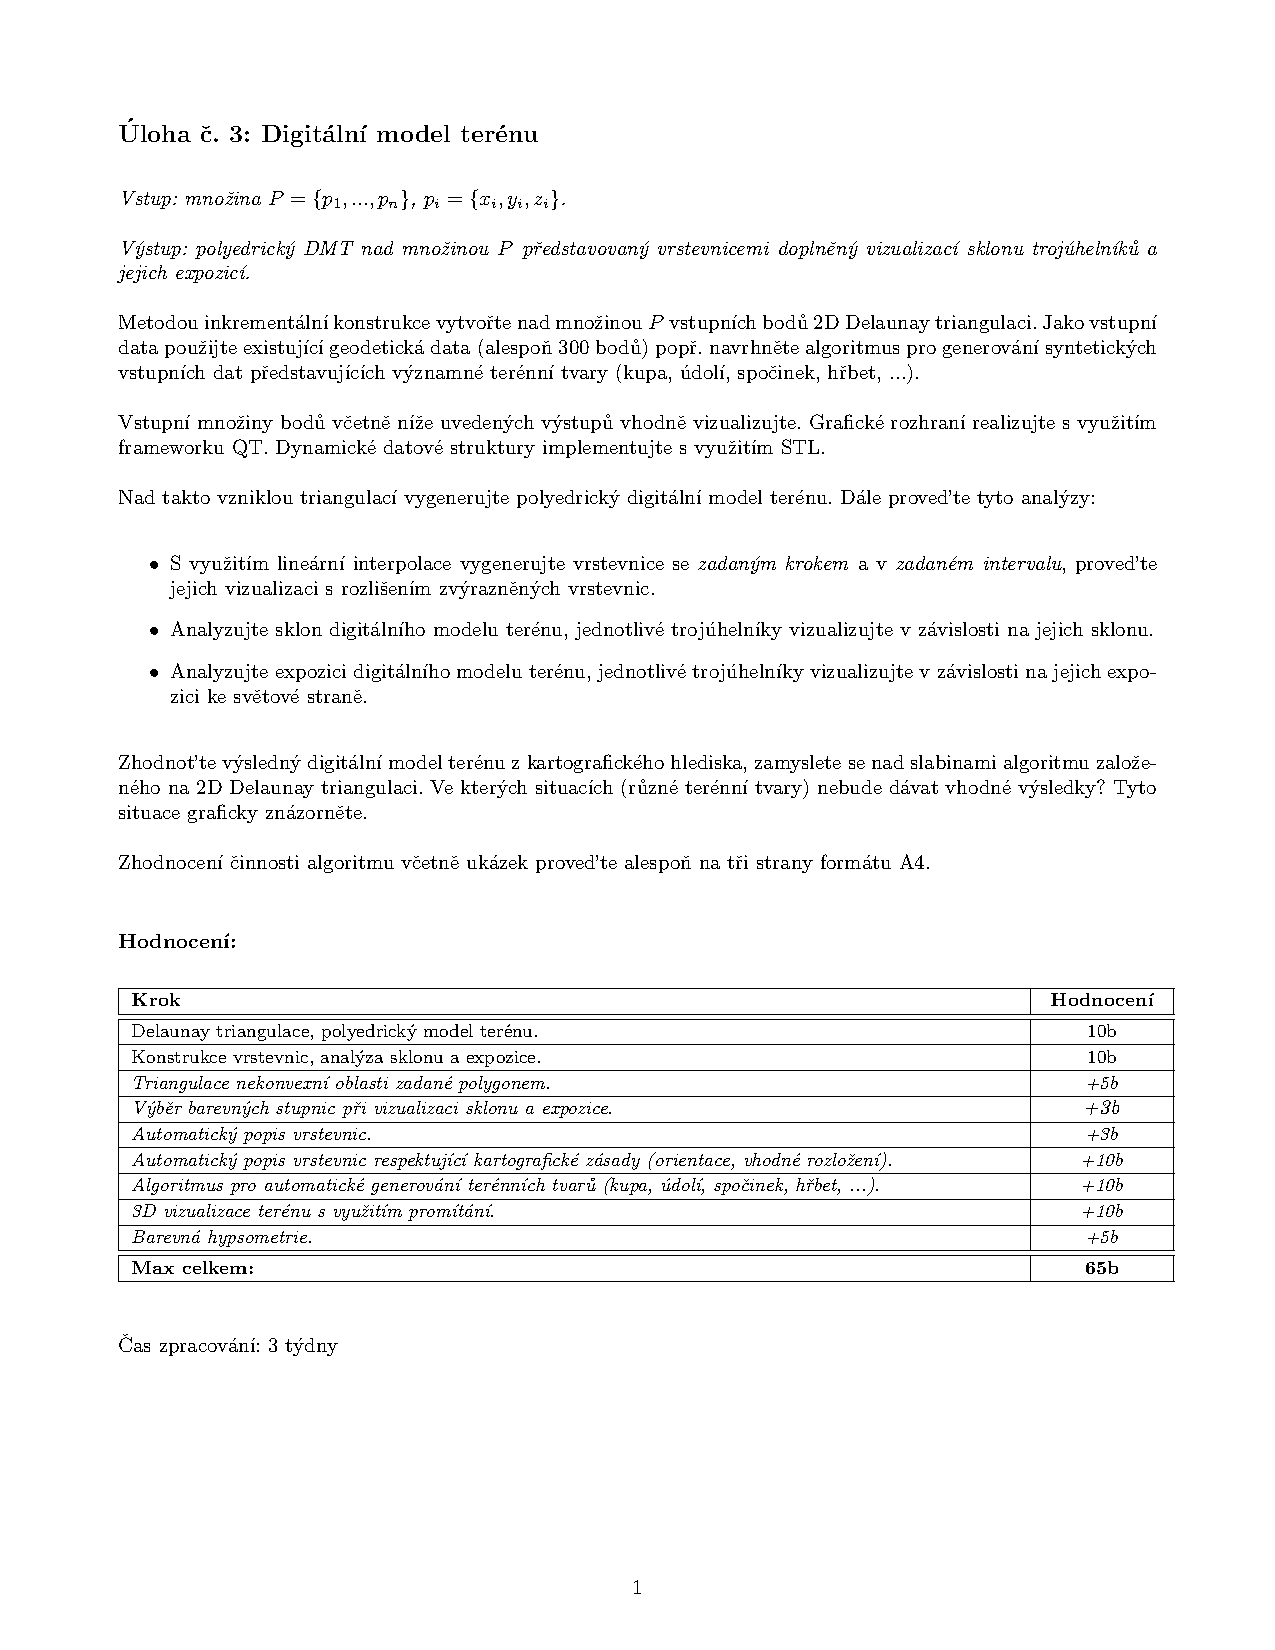
\includepdf[scale=0.9,pages=1,pagecommand=\section{Zadání}]{zadani.pdf}
\section{Popis a rozbor problému} %+vzorce
\indent Výstupem je program, který dokáže vytvořit nad prostorovou množinou DMT pomocí triangulace, vrstevnice a vizualizovat sklon terénu a jeho expozici. 

\section{Popisy algoritmů} %formálním jazykem
\subsection{Delaunay triangulace}
\indent Delaunay triangulace je nejčastěji používanou triangulací v oblasti GIS, lze jí provádět jak plošně, tak prostorově. \\
\textbf{Podmínky DLT}
\begin{itemize}
	\item Uvnitř kružnice v libovolném trojúhelníku triangulace neleží žádný jiný bod množiny.
	\item Tato triangulace maximalizuje minimální úhel v trojúhelníku, avšak neminimalizuje maximální úhel.
	\item Je lokálně i globálně optimální vůči kritériu minimálního úhlu. 
	\item Triangulace je jednoznačná, pokud žádné čtyři body neleží na kružnici.
\end{itemize}
\indent Triangulace byla realizována metodou inkrementální konstrukce. Tato metoda je založena na postupném přidávání bodů do již vytvořené triangulace. Hledá se takový bod, který má spolu s dvěma body triangulace nejmenší opsanou kružnici. Každá hrana trojúhelníku je orientována a body hledáme pouze vlevo od ní. \\
\indent Pokud je nalezen vyhovující bod, jsou do výsledné triangulace přidány orientované hrany nového trojúhelníku. Pokud neexistuje žádný takový bod, změníme orientaci hrany a hledání opakujeme. \\
\indent Pro ukládání hran se používá tzv. \textit{Active Edge List}. Tato struktura obsahuje hrany, ke kterým hledáme třetí bod. Když je třetí bod k hraně nalezen, hrana je odebrána ze seznamu. Následně se kontroluje, zda není v AEL tato hrana již přítomna s opačnou orientací. Pokud je, je z tohoto seznamu odstraněna. Pokud není, je hrana do AEL naopak přidána. V každém případě je ale hrana přidána do výsledné triangulace. Takto se v algoritmu postupuje, dokud není AEL prázdný. 
\subsection{Vrstevnice}
\indent Vrstevnice byly počítány pomocí lineární interpolace. U lineární interpolace je rozestup mezi dvěma body konstantní, spád terénu taktéž. \\
\indent Princip spočívá ve vyhledání průsečnice roviny určené postupně každým trojúhelníkem a roviny vodorovné se zadanou výškou \textit{h}, ve které chceme bod vrstevnice nalézt. \\
\indent Zda protíná rovina stranu trojúhelníku lze zjistit jednoduchým testem:
$(z-z_i)(z-z_{i+1}))<0$.
\indent Pokud je průsečnicí těchto rovin úsečka, vypočítají se souřadnice jejích bodů následovně:
$$ x_a = \frac{(x_3-x_1)}{z_3-z_1}(z-z_1)+x_1, $$
$$y_a = \frac{(y_3-y_1)}{z_3-z_1}(z-z_1)+y_1,$$
$$ x_b = \frac{(x_2-x_1)}{z_2-z_1}(z-z_1)+x_1, $$
$$y_b = \frac{(y_2-y_1)}{z_2-z_1}(z-z_1)+y_1.$$
\subsection{Počítání sklonu} 
\indent Výpočet sklonu se provádí nad každým trojúhelníkem v DMT. Trojúhelník je jasně daný dvěma vektory, odchylka $\varphi$ dvou rovin se spočte následovně: 
$$\varphi = \arccos(\frac{n_1n_2}{|n_1n_2|}).$$
\subsection{Orientace svahu}
\indent Orientace svahu v bodě je definována jako azimut $A$ průmětu gradientu $\bigtriangledown\rho(x_0,y_0,z_0)$ do roviny $xy$, který se spočte jako
$$A = \arctan(\frac{n_1}{n_2}), A\in\langle0,2\pi),$$
kde $n_1, n_2$ jsou vektorové součiny vektorů, které tvoří daný trojůhelník.

\section{Vstupní data}
\indent Do programu lze načíst soubor ve formátu \textit{*.txt}, který na každém řádku obsahuje XYZ souřadnice jednoho vkládaného bodu: \\
\texttt{
54625.84 23547.74 250.5 \\
54826.52 23580.78 266.7 \\
54752.66 23612.32 245.8 \\
.\\
.\\
.}
\section{Výstupní data}
\indent Program načte vstupní data a po stisku tlačítka \textit{Delaunay triangulation} vykreslí body a jejich triangulaci. Při každém vykreslení triangulace se aktualizuje šířka okna a podle té se pak body natransformují a zobrazí.
\indent Poté si uživatel může zvolit, zda chce vizualizaci vrstevnic (tlačítko \textit{Contour lines}) - zde je potřeba si nastavit požadovaný interval a rozmezí, ve kterém se vrstevnice generují (pro orientaci vidí uživatel výšku nejnižšího a nejvyššího z načtených bodů). Také lze barevně zobrazit sklon terénu (\textit{Slope}) a  jeho orientaci (\textit{Orientation}). Pro vyčištění plochy a ponechání pouze načtených bodů slouží tlačítko \textit{Clear}. \\


\section{Ukázky aplikace} %printscreen
\indent Vzhledem k nejasné chybě v algoritmu pro triangulaci je tato kapitola omezená jen na ukázku vzhledu UI a vykreslení vrstevnic. \\
\begin{figure}[htbp]
\centering
        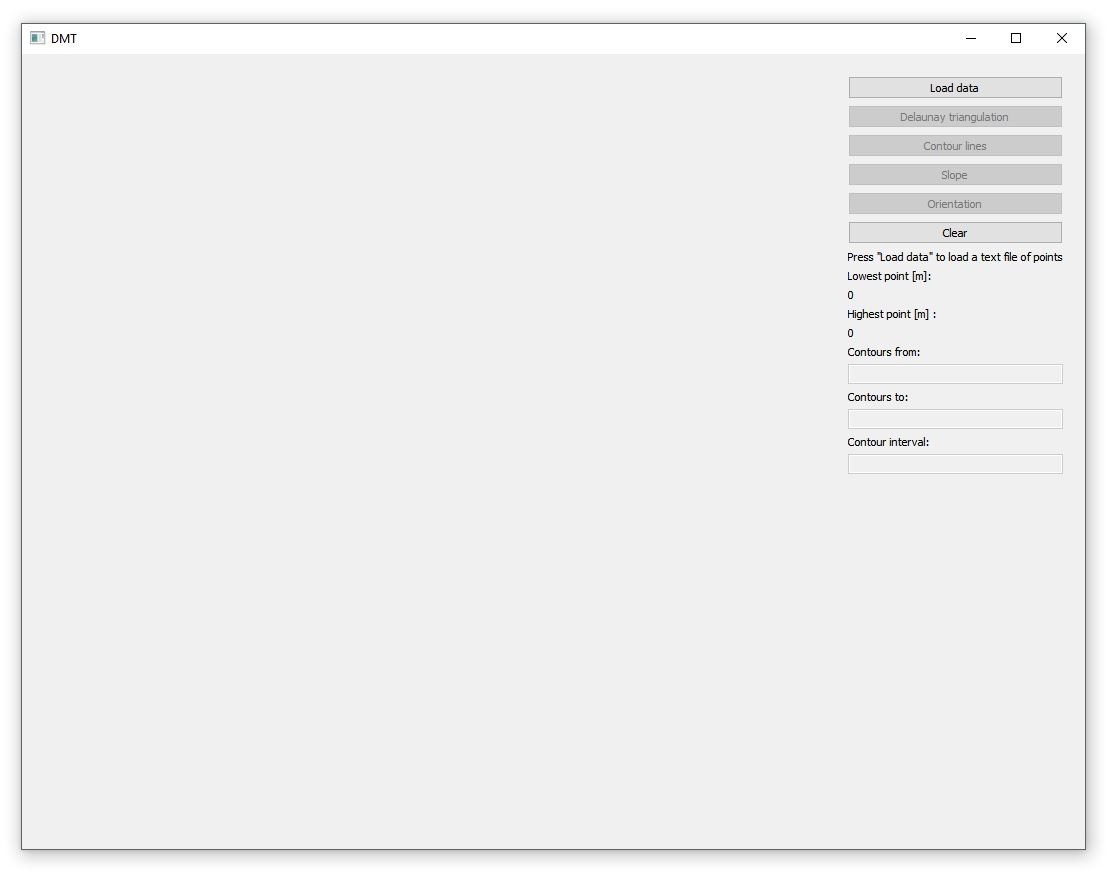
\includegraphics[trim=0cm 0cm 0cm 0cm, width=1\textwidth]{startup.jpg}
        \caption{Vzhled aplikace při otevření}
\end{figure}

\begin{figure}[htbp]
\centering
        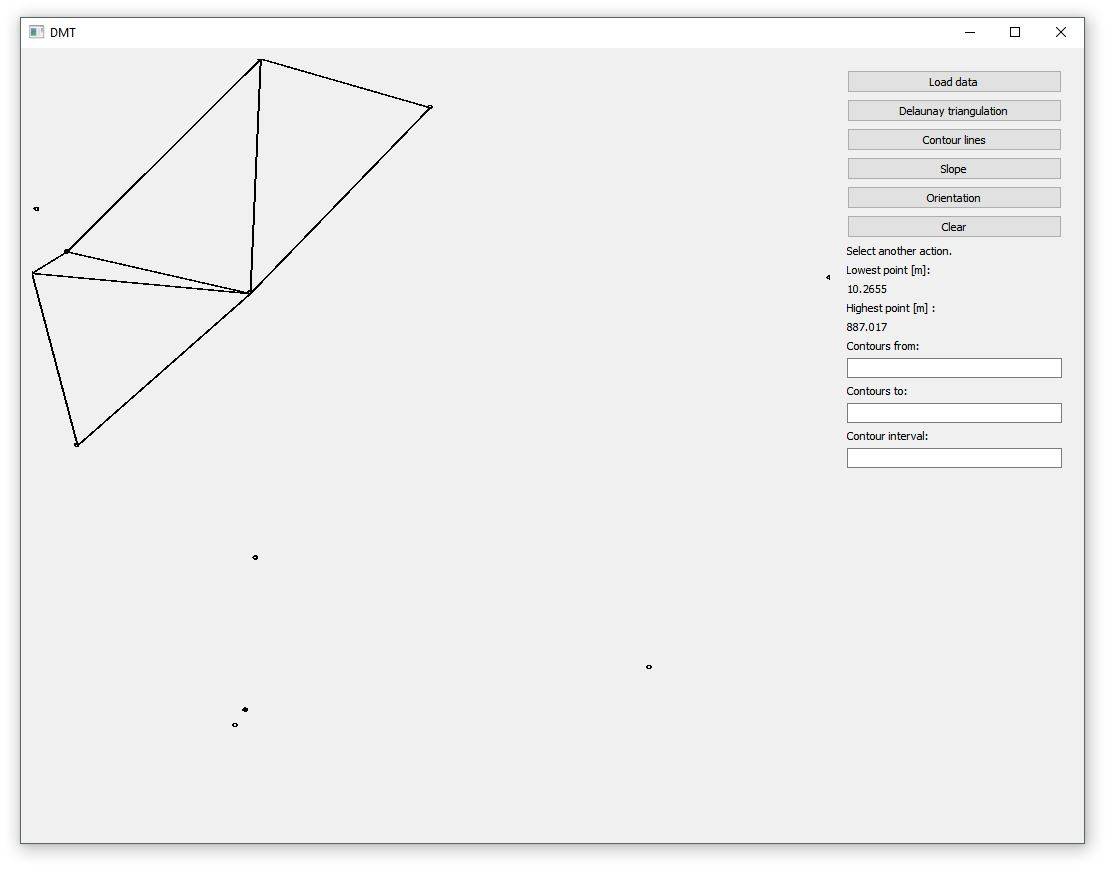
\includegraphics[trim=0cm 0cm 0cm 0cm, width=1\textwidth]{triangulate.jpg}
        \caption{Aplikace po provedení triangulace}
\end{figure}

\begin{figure}[htbp]
\centering
        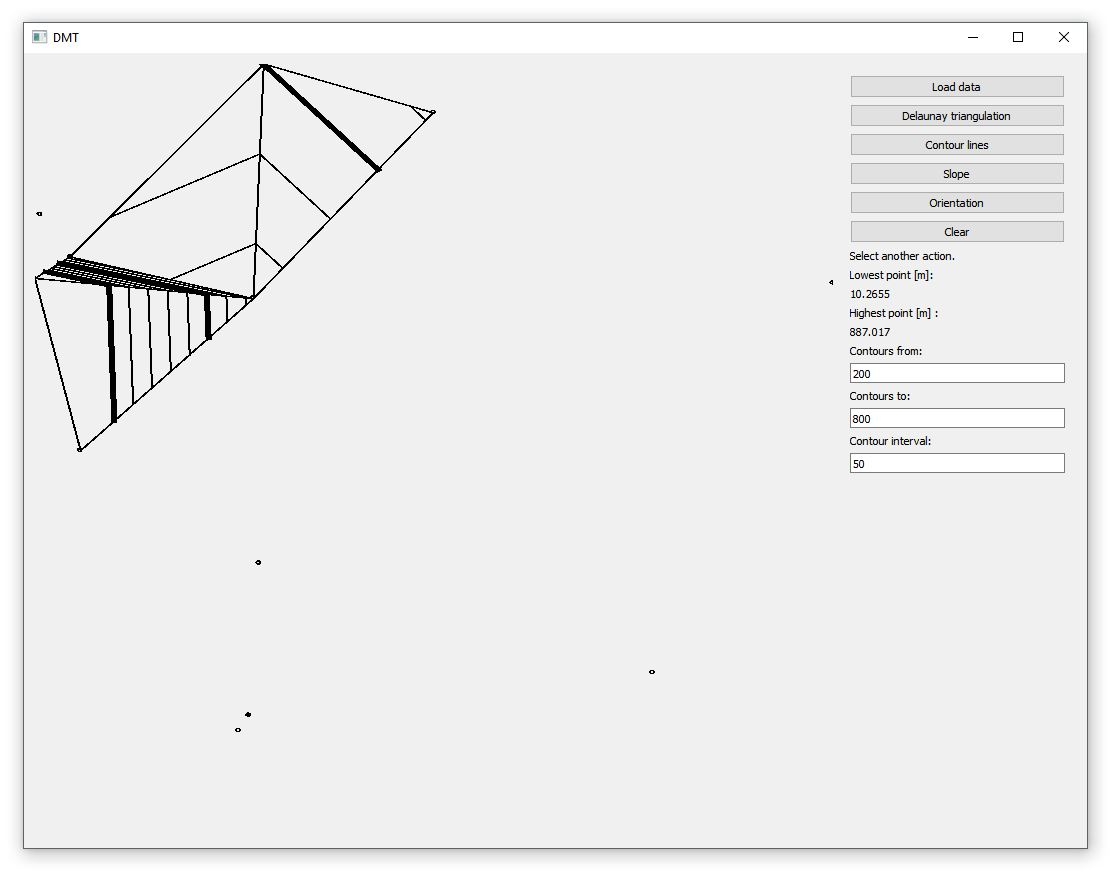
\includegraphics[trim=0cm 0cm 0cm 0cm, width=1\textwidth]{contours.jpg}
        \caption{Aplikace po zobrazení vrstevnic}
\end{figure}

\section{Závěr}
Byla vytvořena aplikace, která nad Delaunay triangulací počítá a zobrazuje sklon, vrstevnice a orientaci svahu. Aplikace má pár nedostatků, které již bohužel autoři nestihli opravit.
	\subsection{Náměty na vylepšení} %+možné či neřešené problémy
	V aplikaci je několik problému, které jsou vyřešeny špatně a bohužel nezbyl čas je opravit. Mezi tyto chyby patří: 
	\begin{itemize}
	\item Špatné počítání sklonu - barva by se měla údajně měnit v různých stupních šedi.
	\item Špatný výpočet orientace - při každém překreslení dává jiné výsledky.
	\item Špatné zadávání velkého množství dat - z autorce neznámého důvodu program zvládá načíst menší soubor s ručně psanými daty, ale data převzatá od kolegy Bc. Bucka a upravená autorem načíst nelze. Autorka se domnívá, že je problém buď ve formátu převzatých dat nebo v načítání, které by mohlo být zbytečně pomalé a zdlouhavé. Bohužel nezbyl čas na to zjistit, o kterou z těchto dvou příčin by se mohlo jednat. 
	\end{itemize}
	
%\pagestyle{empty}

%\end{homeworkSection}
\clearpage

%-----------------------------------------------------------------------------
\end{document}